\section{Feasibility Study}

A feasibility study is an assessment of the practicality of a proposed project or system. A feasibility study aims to objectively and rationally uncover the strengths and weaknesses of an existing business or proposed venture, opportunities and threats present in the natural environment, the resources required to carry through, and ultimately the prospects for success. In its simplest terms, the two criteria to judge feasibility are cost required and value to be attained. A well-designed feasibility study should provide a historical background of the business or project, a description of the product or service, accounting statements, details of the operations and management, marketing research and policies, financial data, legal requirements and tax obligations. Generally, feasibility studies precede technical development and project implementation.

A feasibility study evaluates the project’s potential for success; therefore, perceived objectivity is an important factor in the credibility of the study for potential investors and lending institutions. It must therefore be conducted with an objective, unbiased approach  to provide information upon which decisions can be based. Taking into consideration the technical, operational and economic feasibility as below, the project can be anticipated as feasible overall. There are few types of feasibility that exists. So, developers should take care of these feasibility and take them into consideration:


\subsection{Technical Feasibility}
This assessment is based on an outline design of system requirements, to determine whether the company has the technical expertise to handle completion of the project. At this level, the concern is whether the proposal is both technically and legally feasible (assuming moderate cost). It is an evaluation of the hardware and software and how it meets the need of the proposed system.

This project is built upon Jupyter Notebook, a simple Web-Application or CLI with Python as the programming language and can be easily hosted on cloud server. Also all the other technologies used are capable of building such a project and serve as well as maintain it for longer period of time. All the required hardware and software are easily available in the market. Hence the project is technically feasible.




\subsection{Operational Feasibility}
Operational feasibility is the measure of how well a proposed system solves the problems, and takes advantage of the opportunities identified during scope definition and how it satisfies  the requirements identified in the requirements analysis phase of system development.

The operational feasibility assessment focuses on the degree to which the proposed development project fits in with the existing business environment and objectives with regard to development schedule, delivery date, corporate culture and existing business processes. The application is operationally feasible since it is build with the idea for integration with various existing applications and systems.


\subsection{Economical Feasibility}
Describes how much time is available to build the new system, when it can be built, whether it interferes with normal business operations, type and amount of resources required, dependencies, and developmental procedures with company revenue prospectus.

As the necessary hardware and the software are easily available in the market at low cost, the initial investment is the only cost incurred and does not need further enhancement. Hence it is economically feasible.


\section{Risk Analysis}
Risk Analysis and Management is a key project management practice to ensure that the least number of surprises occur while your project is underway. While we can never predict the future with certainty, we can apply a simple and streamlined risk management process to predict the uncertainties in the projects and minimize the occurrence or impact of these uncertainties.

This project has a very slight window for experiencing failures not in technical aspects but those functionalities involving real life interaction might be affected. 

\section{Project Scheduling}
Generally, project scheduling can be stated as the estimated time required for any project from its time of beginning to the end of the project. In detail, for every task, there is a deadline because all the tasks for the completion of project are planned earlier. So that, each task is scheduled to certain time limit.   15 In short, in project management, listing of projects milestones, activities and all from starting to end date, are considered in the project scheduling. A schedule is generally used in the project planning and management of the project with some kind of attributes as budget, task allocation and duration, resource allocation and all.
 \begin{table}[H]
     \centering
     \begin{tabular}{c|c}
         
         \begin{tabularx}{1\textwidth} { 
  | >{\raggedright\arraybackslash}X 
  | >{\raggedright\arraybackslash}X 
  | >{\raggedright\arraybackslash}X|}
 \hline
  Task & Start Date & End Date \\
 \hline
 Selection of title &26 Aug 2022&29 Aug 2022\\
\hline
  Gathering information  &30 Aug 2022&19 Sep 2022\\
\hline
 Project discussion &20 Sep 2022&30 Sep 2022 \\
\hline
  Planning/ requirement gathering and  analysis  &3 Oct 2022&7 Oct 2022 \\
\hline
 Design &7 Oct 2022&14 Oct 2022 \\
\hline
Knowledge and Gathering &17 Oct 2022&2 Dec 2022\\
\hline
Development Phase &5 Dec 2022&11 Jan 2023\\
\hline
Testing &12 Jan 2023&17 Jan 2023\\
\hline
Documentation &26 Aug 2022&15 Mar 2023\\
\hline


\end{tabularx} 
     \end{tabular}
     \caption{Task Scheduling for the project}
     \label{tab:my_label}
 \end{table}
 \begin{figure}[H]
    \centering
    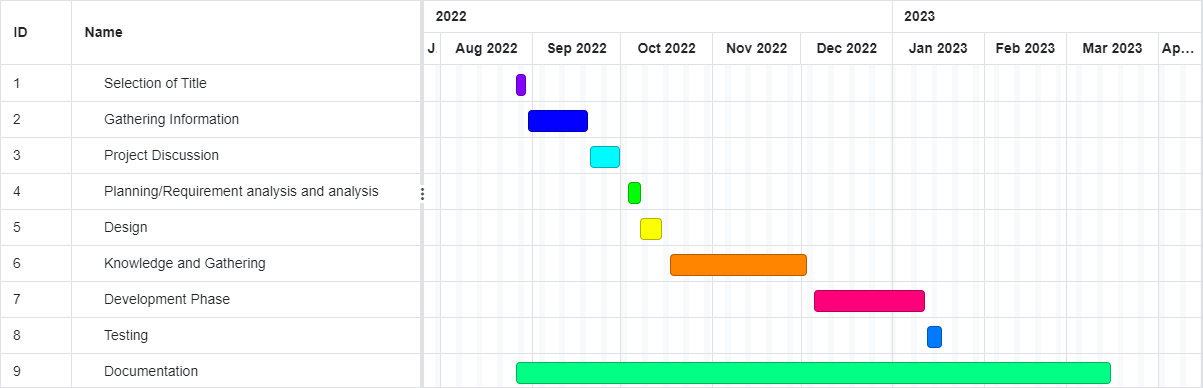
\includegraphics[scale=0.42]{design/Gantt fin.png}
    \caption{Gantt Chart}
    \label{fig:my_label}
\end{figure}    



\section{Effort Allocation}
Effort Allocation is necessary so every team member can give its best to the project. Project was divided into smaller module and task form, for simplification and easy understanding of project overall. Some modules include every team associate’s presence to take advantage of team decision taking skills, and some task include some individual member to work on it with precision. We divided the project into 6 modules.
\begin{itemize}

\item 1.	Gathering of Information
\item 2.	Planning/Requirement Analysis
\item 3.    Selection of Life Cycle
\item 4.	Planning and Management
\item 5.	Analysis & Design UML
\end{itemize}



\begin{table}[H]
    \centering
    \begin{tabular}{c|c}
         \begin{tabularx}{1\textwidth} { 
  | >{\raggedright\arraybackslash}X 
  | >{\centering\arraybackslash}X
  | >{\centering\arraybackslash}X
  | >{\centering\arraybackslash}X
  |>{\centering\arraybackslash}X | }
 \hline
 & Sunidhi & Darshana & Rekha & Lina \\
 \hline
Gathering of information &\checkmark &\checkmark &\checkmark &\checkmark\\
\hline
planning / requirement analysis  &&\checkmark&\checkmark&\\
\hline
 selection of life cycle   &\checkmark&& &\checkmark \\
\hline
planning and management &\checkmark&\checkmark&& \\
\hline
analysis and design &&&\checkmark&\checkmark \\
\hline

\end{tabularx} 
    \end{tabular}
    \caption{Effort Allocation }
    \label{tab:my_label}
\end{table}




\section{Cost Estimation}
Cost Estimation is an important phase for any project. It predicts if the project investment is adequate or there will shortage of capital. It presents the total cost required for development of project. Cost Estimation should be done before initiating the development to prevent loss of efforts and project failure during development. For estimation of cost for this project, we need to consider the server costs for deployment, although the cost is extremely variable since it is dependent on real-time usage.
The cost for a machine learning project is generally calculated in three components i.e. data cost, research cost and production cost. Since our project has the required dataset already available, the data cost for the project is zero. The research cost is dependent on the number of people involved in the project for the amount of time required for the project. Assuming the cost for each person who does research to be Rs. 20000 per month, if 4 people work for a timeline of 6 months, the research cost will be\\

Research Cost = 4 people x 6 months x Rs. 20000\\
= Rs. 4,80,000\\

According to the Google Cloud Calculator, the cost for deploying an E2 compute engine with Windows as operation system, 4 vCPU’s and 16 GB RAM is Rs. 7000 per month. If the deployment is to be done for 12 months, the production cost will be
 
Production Cost = 12 months x Rs. 7000\\
= Rs. 84,000

Hence the total cost of the project can be calculated as

Total Cost = Research Cost + Production Cost\\
= Rs. 4,80,000 + Rs. 84,000\\
Total Cost = Rs. 5,64,000


\section{Summary}
The project, is hence found to be feasible since there is a balance of resources required and the cost incurred. Also the project helps the government to identify crime like child labour. The project will be able to easily integrate with other required systems.